%==================== BENCH4Q
\begin{frame}{Bench4Q}

\begin{itemize}
\item Bench4Q e um \textit{benchmark} para avaliação de desempenho em regime estacionário.

\item Não existem provisões para a introdução de perturbações programadas durante o experimento.

\item Código fonte disponível~\footnote{http://www.trustie.net/projects/project/show/Bench4Q}.

\item Amplamente utilizado na literatura~\footnote{\cite{Wang2012b,Zhang2012a,Gao2013}}.
\end{itemize}


\end{frame}

\begin{frame}{Características}

Bench4Q:
\begin{itemize}
	\item É uma extensão do \textit{benchmark} \textbf{TPC-W} \cite{Garcia2003}.
	\item Suporta analise de métricas baseadas em sessões.
	\item A geração de carga é baseada em agentes:
	\begin{itemize}
		\item Cada agente disponibiliza vários \textit{Workers} ou EBs (\textit{Emulate Browsers}).
		\item Agentes locais ou remotos.
	\end{itemize}
	\item Utiliza uma loja de livros: \textit{Software Under Test} (\textbf{SUT}).
\end{itemize}

\end{frame}

\begin{frame}{Caraterísticas}
	\begin{figure}
		\begin{center}
			\includegraphics[scale=0.35]{images/sut.png}
			\caption{Bench4Q: SUT.}
			\label{fig:sut-bench4q}
		\end{center}
	\end{figure}
\end{frame}


\begin{frame}{Métricas disponíveis no Bench4Q}
%Métricas de interesse disponíveis no Bench4Q:
\begin{itemize}
	\item WIRT (\textit{Web Interaction Response Time})
	\item WIPS (\textit{Web Interacton Per Second})
	\item VSPS (\textit{Valid Sessions Per Second})
	\item VSR (\textit{Valid Sessions Ratio})	
\end{itemize}

\end{frame}

\begin{frame}{Métricas disponíveis no Bench4Q}
\begin{figure}
	\begin{center}
		\includegraphics[scale=0.5]{images/metricas.png}
			\caption{Bench4Q: Métrica VSPS.}
					\label{fig:vsps-bench4q}
	\end{center}
\end{figure}

\end{frame}

\begin{frame}{Arquitetura Bench4Q}
	\begin{figure}
		\begin{center}
			\includegraphics[scale=0.2]{images/bench4Q.png}
			\caption{Arquitetura Bench4Q \cite{Bench4Q}.}
			\label{fig:arquitetura-bench4q}
		\end{center}
	\end{figure}
\end{frame}

\begin{frame}{Gerador de carga}
  \putat{150}{-120,5}{
  	\includegraphics[scale=0.4]{images/console-bench4Q.png}
  }
\begin{itemize}
\item Tipos de navegação:
\begin{enumerate}
	\item \textit{Browsing}
	\item \textit{Ordering}
	\item \textit{Shopping}
\end{enumerate}
%\item Gerenciamento dos agentes.
\end{itemize}  


\end{frame}

\begin{frame}{Comportamento dos EBs}
CBMG (\textit{Customer Behavior Model Graph}) é um grafo estatístico que modela o comportamento de navegação de um usuário(emulado).

	\begin{figure}
		\center
		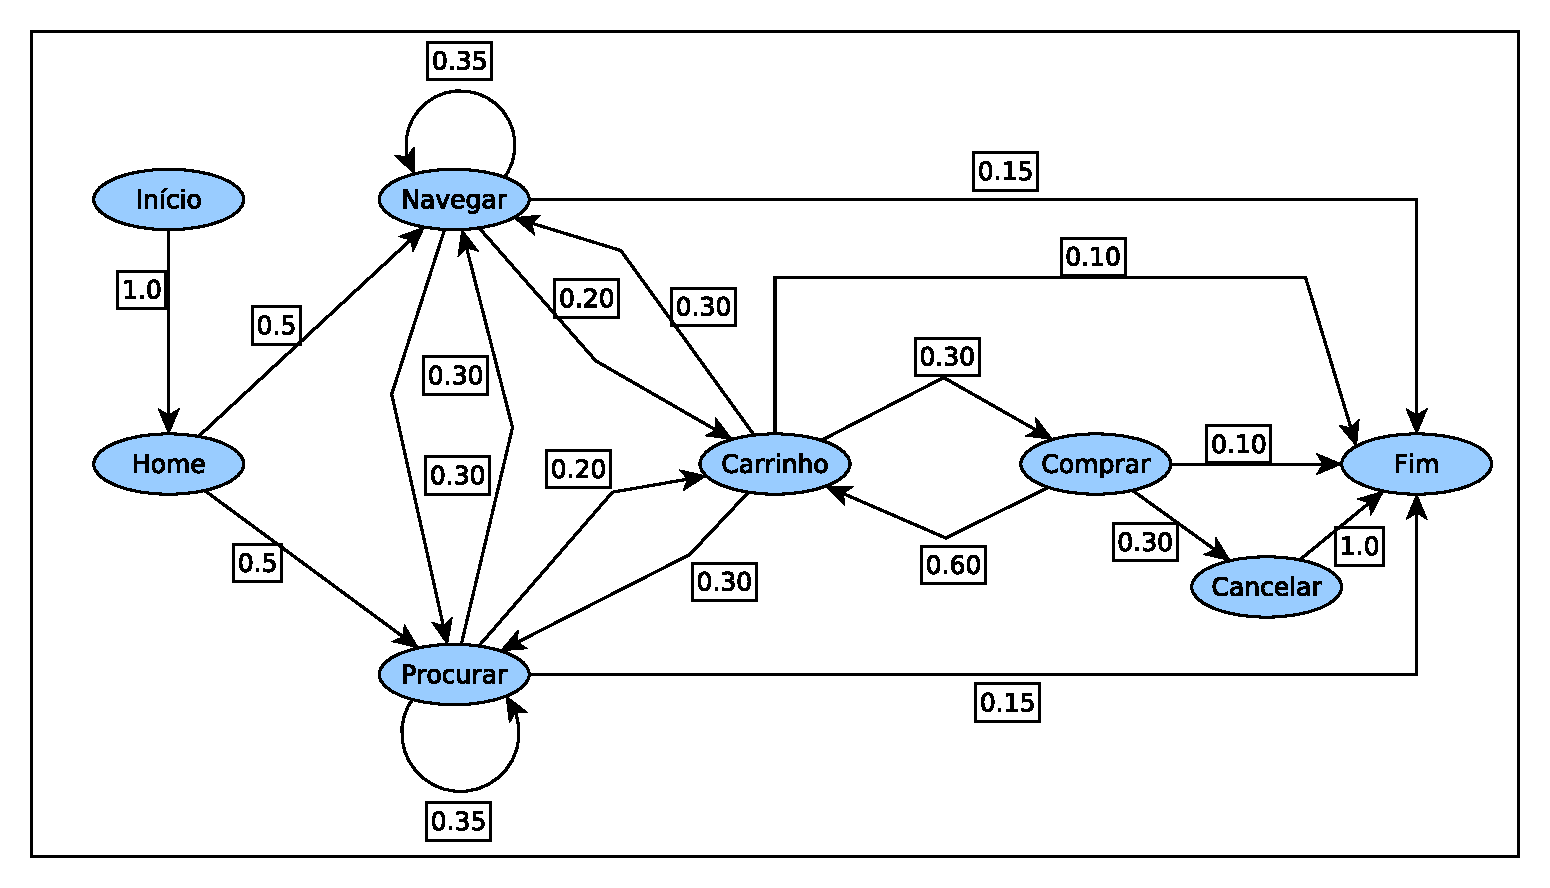
\includegraphics[scale=0.35]{images/CBMG}
		\caption{Perfil interação estocástico com o sistema (SUT).}
		\label{fig:CBMG}
	\end{figure}
\end{frame}